%%%%%%%%%%%%%%%%%%%%%%%%%%%%%%%%%%%%%%%%% 
% Beamer Presentation
% LaTeX Template
% Version 1.0 (10/11/12)
% 
% This template has been downloaded from:
% http://www.LaTeXTemplates.com
% 
% License:
% CC BY-NC-SA 3.0 (http://creativecommons.org/licenses/by-nc-sa/3.0/)
% 
%%%%%%%%%%%%%%%%%%%%%%%%%%%%%%%%%%%%%%%%% 

% ----------------------------------------------------------------------------------------
%	PACKAGES AND THEMES
% ----------------------------------------------------------------------------------------

\documentclass{beamer}

\mode<presentation> {

  % The Beamer class comes with a number of default slide themes
  % which change the colors and layouts of slides. Below this is a list
  % of all the themes, uncomment each in turn to see what they look like.

  % \usetheme{default}
  % \usetheme{AnnArbor}
  % \usetheme{Antibes}
  % \usetheme{Bergen}
  % \usetheme{Berkeley}
  % \usetheme{Berlin}
  % \usetheme{Boadilla}
  % \usetheme{CambridgeUS}
  % \usetheme{Copenhagen}
  % \usetheme{Darmstadt}
  % \usetheme{Dresden}
  % \usetheme{Frankfurt}
   \usetheme{Goettingen}
  % \usetheme{Hannover}
  % \usetheme{Ilmenau}
  % \usetheme{JuanLesPins}
  % \usetheme{Luebeck}
  % \usetheme{Madrid}
  % \usetheme{Malmoe}
  % \usetheme{Marburg}
  % \usetheme{Montpellier}
  % \usetheme{PaloAlto}
  % \usetheme{Pittsburgh}
  % \usetheme{Rochester}
  % \usetheme{Singapore}
  % \usetheme{Szeged}
  % \usetheme{Warsaw}

  % As well as themes, the Beamer class has a number of color themes
  % for any slide theme. Uncomment each of these in turn to see how it
  % changes the colors of your current slide theme.

  % \usecolortheme{albatross}
  % \usecolortheme{beaver}
  % \usecolortheme{beetle}
  % \usecolortheme{crane}
  % \usecolortheme{dolphin}
  % \usecolortheme{dove}
  % \usecolortheme{fly}
  % \usecolortheme{lily}
  % \usecolortheme{orchid}
  % \usecolortheme{rose}
  % \usecolortheme{seagull}
  % \usecolortheme{seahorse}
  % \usecolortheme{whale}
  % \usecolortheme{wolverine}

  % \setbeamertemplate{footline} % To remove the footer line in all slides uncomment this line
   \setbeamertemplate{footline}[page number] % To replace the footer line in all slides with a simple slide count uncomment this line

  % \setbeamertemplate{navigation symbols}{} % To remove the navigation symbols from the bottom of all slides uncomment this line
}

\usepackage{graphicx} % Allows including images
\usepackage{booktabs} % Allows the use of \toprule, \midrule and \bottomrule in tables
\usepackage[german]{babel} % Required to compile in Windows
\usepackage[latin1]{inputenc}
\usepackage{caption}
\usepackage{subcaption}
%\usepackage{physics}
\usepackage{mathtools}
\usepackage{natbib}
\usepackage[T1]{fontenc}


\AtBeginSection[]{
  \begin{frame}
    \vfill
    \centering
    \begin{beamercolorbox}[sep = 8pt, center, shadow = true, rounded = true]{title}
      \usebeamerfont{title}\insertsectionhead\par%
    \end{beamercolorbox}
    \vfill
  \end{frame}
}

% ----------------------------------------------------------------------------------------
%	TITLE PAGE
% ----------------------------------------------------------------------------------------

\title[]{Sehr gute Wetterstation: Die Projektvorstellung} % The short title appears at the bottom of every slide, the full title is only on the title page

\author{Isabell Albrecht, Erik Engelhardt, Oliver Kochan, Florian Steffens} % Your name
\institute[HAW] % Your institution as it will appear on the bottom of every slide, may be shorthand to save space
{
  Hochschule f�r angewandte Wissenschaften -- Hamburg \\ % Your institution for the title page
  \medskip
  \textit{erik.engelhardt@haw-hamburg.de, hier@email.eintragen} % Your email address
}

\date{\today} % Date, can be changed to a custom date

\begin{document}

\begin{frame}
  \titlepage % Print the title page as the first slide
\end{frame}

\section{Einleitung}
% - Gruppenmitglieder vorstellen
% - welches Projekt bearbeiten wir (Bild)
\begin{frame}
  \frametitle{Folie 1}
  \emph{Diese Wetterstation wird sehr gut.}
\end{frame}

\begin{frame}[allowframebreaks]
  %\frametitle{Gliederung} % Table of contents slide, comment this block out to remove it
  \tableofcontents % Throughout your presentation, if you choose to use \section{} and \subsection{} commands, these will automatically be printed on this slide as an overview of your presentation
\end{frame}

% ----------------------------------------------------------------------------------------
%	PRESENTATION SLIDES
% ----------------------------------------------------------------------------------------

\section{Anforderungen}
% - zusammenfassen der Puntke aus Vorlage
% - eingrenzung Messbereiche
\begin{frame}
  \frametitle{Folie 1}
  \emph{Diese Wetterstation wird sehr gut.}
\end{frame}
\section{Konzept}
% - Blockschaltbild
\begin{frame}
  \frametitle{Folie 1}
  \emph{Diese Wetterstation wird sehr gut.}
\end{frame}
\section{Umsetzung}
% - Sensoren kurz vorstellen und Bezug auf Anforderungen nehmen
\begin{frame}
  \frametitle{Sensoren}
  \subsection{Sensoren}
        Messwerterfassung
        \begin{itemize}
            \item \emph{Bosch Sensortec} \href{https://www.bosch-sensortec.com/bst/products/all_products/bme280}{\textbf{BME280}}: Luftdruck-, Luftfeuchte- und Temperatursensor
            \item \emph{Honeywell} \href{https://www.sparkfun.com/datasheets/Components/HMC6352.pdf}{\textbf{HMC6352}}: Magnetometer mit DSP-ASIC
            \item \emph{ST Microelectronics} \href{https://www.st.com/en/mems-and-sensors/lis3dh.html}{\textbf{LIS3DH}}: MEMS-Accelerometer und Temperatursensor
            \item \emph{Allegro} \href{https://www.allegromicro.com/en/products/sense/current-sensor-ics/zero-to-fifty-amp-integrated-conductor-sensor-ics/acs712}{\textbf{ACS712}}: Halleffekt-Stromsensor
            \item \emph{Sparkfun} \href{https://www.sparkfun.com/products/8942}{\textbf{SEN-08942}}: Anemometer, Windfahne und Niederschlagssensor
        \end{itemize}
\end{frame}
\begin{frame}
    \frametitle{Kommunikation und Leistungselektronik}
    \subsection{Kommunikation, LE}
        Kommunikations- und Leistungselektronik:
        \begin{itemize}
            \item \emph{SkyTraq} \href{}{\textbf{Venus600 series}}: GPS Empf�nger-ASIC
            \item \emph{``no-name''} \textbf{HC-05}: Serial-over-Bluetooth Schnittstellenumsetzer
            \item \emph{ST Microelectronics} \href{https://www.st.com/en/motor-drivers/l293e.html}{\textbf{L293E}}: Motortreiber
            \item \emph{IVT} \textbf{200007}: MPPT Laderegler
        \end{itemize}
\end{frame}
\begin{frame}
\frametitle{Energieversorgung}
    \subsection{Versorgung}
        Autarke Energieversorgung:
        \begin{itemize}
            \item \emph{Sygonix} \textbf{SY-VRU214-4}: Solarmodul
            \item\emph{``no-name''} Blei-S�ure Sekund�rzelle
        \end{itemize}
\end{frame}
\begin{frame}
\frametitle{System�bersicht}
    \subsection{Aufbau}
        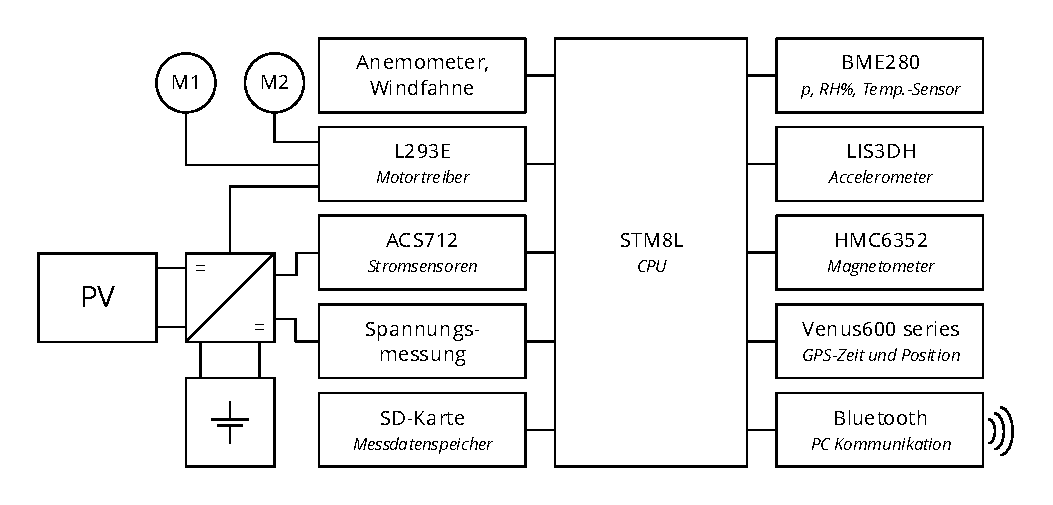
\includegraphics[width=\textwidth]{img/BSB_Uebersicht.pdf}
\end{frame}
\section{Zeitplan}
% - groben Zeitplan vorstellen (Diagramm)
\begin{frame}
  \frametitle{Folie 1}
  \emph{Diese Wetterstation wird sehr gut.}
\end{frame}

\begin{frame}[allowframebreaks]
  \frametitle{Literatur- und Quellenverzeichnis}
  \bibliographystyle{plainnat}
  \bibliography{literature}
\end{frame}

% ------------------------------------------------
% ----------------------------------------------------------------------------------------

\end{document}
%%% Local Variables:
%%% mode: latex
%%% TeX-master: t
%%% End:
